%%%%%%%%%%%%%%%%%%%%%%%%%%%%%%%%%%%%%%%%%
% Short Sectioned Assignment
% LaTeX Template
% Version 1.0 (5/5/12)
%
% This template has been downloaded from:
% http://www.LaTeXTemplates.com
%
% Original author:
% Frits Wenneker (http://www.howtotex.com)
%
% License:
% CC BY-NC-SA 3.0 (http://creativecommons.org/licenses/by-nc-sa/3.0/)
%
%%%%%%%%%%%%%%%%%%%%%%%%%%%%%%%%%%%%%%%%%

%----------------------------------------------------------------------------------------
%	PACKAGES AND OTHER DOCUMENT CONFIGURATIONS
%----------------------------------------------------------------------------------------

\documentclass[paper=a4, fontsize=11pt]{scrartcl} % A4 paper and 11pt font size

\usepackage[T1]{fontenc} % Use 8-bit encoding that has 256 glyphs
\usepackage{fourier} % Use the Adobe Utopia font for the document - comment this line to return to the LaTeX default
\usepackage[english]{babel} % English language/hyphenation
\usepackage{amsmath,amsfonts,amsthm} % Math packages
\usepackage{graphicx}
\usepackage{tikz}
\usetikzlibrary{arrows}
\usetikzlibrary{positioning}

\usepackage{lipsum} % Used for inserting dummy 'Lorem ipsum' text into the template

\usepackage{sectsty} % Allows customizing section commands
\allsectionsfont{\centering \normalfont\scshape} % Make all sections centered, the default font and small caps

\usepackage{fancyhdr} % Custom headers and footers
\pagestyle{fancyplain} % Makes all pages in the document conform to the custom headers and footers
\fancyhead{} % No page header - if you want one, create it in the same way as the footers below
\fancyfoot[L]{} % Empty left footer
\fancyfoot[C]{} % Empty center footer
\fancyfoot[R]{\thepage} % Page numbering for right footer
\renewcommand{\headrulewidth}{0pt} % Remove header underlines
\renewcommand{\footrulewidth}{0pt} % Remove footer underlines
\setlength{\headheight}{13.6pt} % Customize the height of the header

\numberwithin{equation}{section} % Number equations within sections (i.e. 1.1, 1.2, 2.1, 2.2 instead of 1, 2, 3, 4)
\numberwithin{figure}{section} % Number figures within sections (i.e. 1.1, 1.2, 2.1, 2.2 instead of 1, 2, 3, 4)
\numberwithin{table}{section} % Number tables within sections (i.e. 1.1, 1.2, 2.1, 2.2 instead of 1, 2, 3, 4)

\setlength\parindent{0pt} % Removes all indentation from paragraphs - comment this line for an assignment with lots of text

%----------------------------------------------------------------------------------------
%	TITLE SECTION
%----------------------------------------------------------------------------------------

\newcommand{\horrule}[1]{\rule{\linewidth}{#1}} % Create horizontal rule command with 1 argument of height

\title
{	
\normalfont \normalsize 

\includegraphics[scale=0.7]{feup.png}
\horrule{0.5pt} \\[0.4cm] % Thin top horizontal rule
\huge Project Management with Computational Trust Models in a Multi-Agent Environment\\
\horrule{2pt} \\[0.5cm] % Thick bottom horizontal rule
}

\author{
	Ricardo Ferreira da Silva\\
	\texttt{up201305163@fc.up.pt}
	\and
	Gustavo de Castro Nogueira Pinto\\
	\texttt{up201302828@fe.up.pt}
	\and
	Tiago Filipe Abreu Figueiredo\\
	\texttt{ei12069@fe.up.pt}
}
\date{\normalsize\today} % Today's date or a custom date
\begin{document}

\maketitle % Print the title

%----------------------------------------------------------------------------------------
%	PROBLEM 1
%----------------------------------------------------------------------------------------
\newpage

\tableofcontents

\newpage
\section{Objectives}
% and objectives
%------------------------------------------------
A project, in the context of operations research consists of a set of interdependent tasks, a start state and an end state. Each of these tasks has a certain duration and it is required that the tasks preceding it are completed before we can execute it. The start state gives us access to the initial tasks (tasks without precedences), and the final state is reached when all tasks are completed, which means the project itself was completed.

% Maybe example
Expanding upon this context, lets say we are in an simple entrepreneurial setting. A company will certainly have a project which it intends to complete and it possesses a set of workers, each one with a different set of skills and different degrees of proficiency at those skills. There will also exist a very special type of worker, that is, the manager. The manager has the crucial function of evaluating all its subordinate workers and assigning them to the tasks they will be most useful at, with the ultimate objective of finishing the overall project in the shortest amount of time.

Our objective, is to model this problem in an multi-agent environment setting and use computational trust model in order to obtain an evaluation of these workers via a manager, thus obtaining an approximation of the information needed to make the correct choices in terms of allocation.

\section{Specification}
Just as it was described in the previous chapter, the objective of this application is to simulate the development of a project. This project consists of a set of interdependent tasks that must be concluded, a a manager responsible of making decisions and a set of workers, whose ratings are not fully known by the manager.

\subsection{Project Structure}

\subsection{Agents}
In order to model this problem in a multi-agent environment we decided to design three of the main entities in the problem as agents: Manager, Worker and Task. The worker and the task are mostly reactive agents since all their actions are triggered via a manager order, with an exception we will later discuss. The manager is a BDI agent and he is the true "mastermind" so to say behind the project. He has the final objective of finishing the project in the shortest amount of time and he must get to know the worker agents properly so he can effectively allocate them to the available tasks.

\subsubsection{Worker}
In our model a worker is a reactive agent with no autonomy whatsoever. He starts with several pairs of <Skill, Rating> given by the user. These pairs are what allows us to measure how effective a worker will be in a certain task with the following formula, which means the value of a certain worker $w$ to a task $t$.
\begin{center}
	$
	ValueOf(W,T) = 
	\frac
	{\sum\nolimits_{S_i,R_i \in (S \in W \subseteq S \in T )} R_i}
	{|S \in T |}
	$
\end{center}
The worker also contains the set of past <Skill,Value,Reliability> triples, which is were we store the past skill evaluations the Manager made of this worker using the Interaction Trust and Witness Reliability components of FIRE. It also contains the past project ratings, which is where the past evaluations of the worker regarding a particular completed task are stored. Every time a task is completed, the manager will execute the FIRE components on all workers who were working on it. This consists of two FIRE components. The first one is Interaction Trust, which is directly related on the success of task, which means that if the task finished before it was expected, the workers predicted skill ratings will be increased, and if the task finishes after the expected date then the opposite happens. This will allow the manager to fine tune a very good approximation of the workers real skill ratings after a certain number of tasks with different requirements have been executed. The second one is Witness Reliability, which consists in having each worker report the skills of each fellow colleague in that task and give that opinion a weight according to the reliability of that worker. These two components are combined to fabricate the final opinion the manager has on the workers skills. In the beginning Witness Reputation has a higher weight in the equation but it is gradually replaced by Interaction Trust.
\subsubsection{Task}
A task is a reactive agent and it was mostly modelled as such out of convenience due to the capabilities of the platform used. The task is the main entity of the project and all tasks are connected via their dependencies and they always have a state that is either unavailable, available or finished. Every time all the dependencies of a task are finished, that task becomes available which means that is possible to allocate workers in order to finish it. The start state will grant us access to a set of tasks and from there we must finish all tasks in order to reach the end state.

The task agent has several important properties. The expected duration is a value in workers per month that is provided by the user. This means that if the total value of the workers allocated for that task equals the expected duration, then the task will take exactly one month to be completed at that rate.
The set of skills required by the task is also provided by the user in the configuration and it is very important in order to calculate the worth each worker has to that task. Naturally, if the intersection of the workers skills and the tasks skills is empty, then the worker will be worthless (contributes nothing) and might as well be allocated to another task where he might use his skills. Other properties include the completion of the task (0\%-100\%), the rate at which the task progresses per week and the list of currently assigned workers.

The task has one behaviour which is progress task behaviour. This behaviour, which occurs for available tasks being worked on, is triggered every time a week has elapsed (10 ticks in-engine). The execution of this behaviour consists of calculating the rate of progression via total worker value with the following formulas.
\begin{center}
	$\text{Total Worker Worth} = \sum\nolimits_{getWorkerValue(w) + 1}$
\end{center}
\begin{center}
	$\text{Calculated Duration} = \frac{\text{Expected Duration}}{\text{Total Worker Worth}}$
\end{center}
\begin{center}
		$\text{Rate} = \frac
		{100}
		{\text{Calculated Duration}}$
\end{center}
These formulas will give us the percentage of progression each week the task is being worked on. It should be noted that we add 1 in order to convert from the FIRE rating range which is $[-1,1]$ (where -1 is absolutely negative, 0 neutral and 1 absolutely positive), to our own range $[0,\infty]$ which we use for real calculations of task progression.
After the calculations are done, the rate is added to the completion and if it reaches 100\%, then the task is considered complete and the workers are free to work on another task. This behaviour is considered complete when this happens.
\subsubsection{Manager}
The manager is a "Beliefs-Desires-Intentions" type agent that is responsible for allocating the available workers to available tasks with the ultimate goal of finishing the project in the shortest amount of time. The manager has knowledge of all tasks and of all workers. Regarding workers, the manager can order them to work on a task and he does this by deciding if a worker is useful at working in a particular task by comparing his skills and ratings with the skills required by the task. However, when the project starts the manager has no idea what skills (or ratings at those) each worker has, so he assumes each worker to have a neutral value at each skill and that value will be updated using FIRE components each time a task is completed.

The manager has two behaviours. The first one, and also the first behaviour to be executed is the critical path method. The manager takes into account the estimated duration values of each task (provided by the user in the configuration) and their dependencies, calculates the critical time of each task and orders the tasks in a list with this heuristic. This is known has the Critical-Time-Algorithm and while there is no efficient scheduling algorithm currently known that always gives an optimal schedule, the Critical-Time-Algorithm is the best general-purpose scheduling algorithm currently known. Later on, we will describe how we implemented parallel allocation of workers (when there is more than an available task) in order to increase the performance of this algorithm. This behaviour is considered finished after it is executed for the first time.

%reference this --> http://www.ctl.ua.edu/math103/scheduling/scheduling_algorithms.html

The second behaviour, is the available tasks behaviour which is executed every time a task is completed. This behaviour consists in measuring the success (or failure/delay) of the completed task and gathering information about the workers that were working on it via the FIRE components. After this is done, the manager proceeds to analyse the newly freed workers and assign them to the remaining available tasks which maybe entirely new tasks that were unlocked or tasks that are still being worked on by the rest of the workers. It is important to point that while each worker has real rating value for each of his skills, the manager does not know this value. Instead, the manager uses an approximated value that is continuously updated (and approximated to the real value) each time a task is completed. This of course means that the manager might make some poor allocation choices in the beginning of the project due to him not knowing his workers very well, however, as more and more tasks are completed the manager will start having a better approximation of the real skills his workers gave. The manager will continue executing this behaviour, until the final state of the project is reached (when all the tasks are completed).
\section{Development}

\subsection{Platform}

\subsection{Modules}

\subsection{Implementation}
The following graphic is a representation of our class diagram.
\begin{center}
	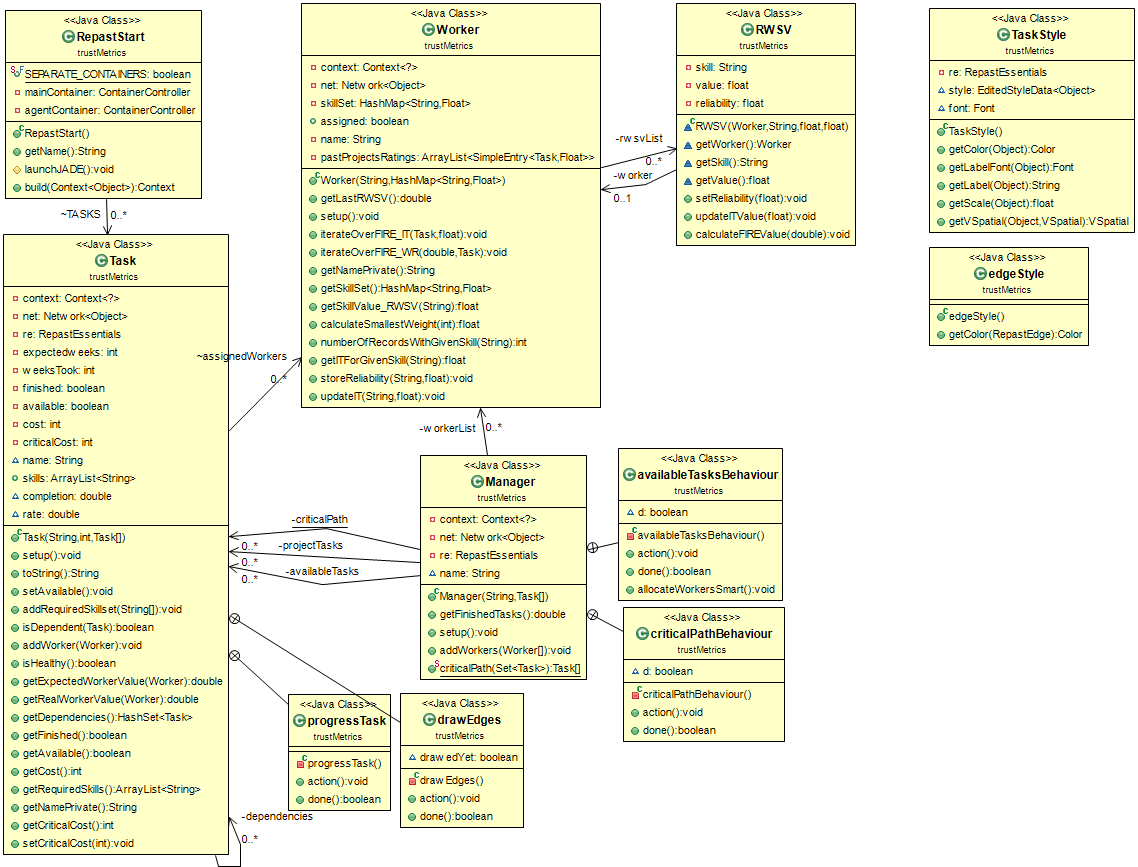
\includegraphics[scale=0.4]{Model.png}
\end{center}
\section{Experiences}

\section{Conclusions}

\section{Improvement}

\end{document}
